%% bare_jrnl.tex
%% V1.4b
%% 2015/08/26
%% by Michael Shell
%% see http://www.michaelshell.org/
%% for current contact information.
%%
%% This is a skeleton file demonstrating the use of IEEEtran.cls
%% (requires IEEEtran.cls version 1.8b or later) with an IEEE
%% journal paper.
%%
%% Support sites:
%% http://www.michaelshell.org/tex/ieeetran/
%% http://www.ctan.org/pkg/ieeetran
%% and
%% http://www.ieee.org/

%%*************************************************************************
%% Legal Notice:
%% This code is offered as-is without any warranty either expressed or
%% implied; without even the implied warranty of MERCHANTABILITY or
%% FITNESS FOR A PARTICULAR PURPOSE! 
%% User assumes all risk.
%% In no event shall the IEEE or any contributor to this code be liable for
%% any damages or losses, including, but not limited to, incidental,
%% consequential, or any other damages, resulting from the use or misuse
%% of any information contained here.
%%
%% All comments are the opinions of their respective authors and are not
%% necessarily endorsed by the IEEE.
%%
%% This work is distributed under the LaTeX Project Public License (LPPL)
%% ( http://www.latex-project.org/ ) version 1.3, and may be freely used,
%% distributed and modified. A copy of the LPPL, version 1.3, is included
%% in the base LaTeX documentation of all distributions of LaTeX released
%% 2003/12/01 or later.
%% Retain all contribution notices and credits.
%% ** Modified files should be clearly indicated as such, including  **
%% ** renaming them and changing author support contact information. **
%%*************************************************************************


% *** Authors should verify (and, if needed, correct) their LaTeX system  ***
% *** with the testflow diagnostic prior to trusting their LaTeX platform ***
% *** with production work. The IEEE's font choices and paper sizes can   ***
% *** trigger bugs that do not appear when using other class files.       ***                          ***
% The testflow support page is at:
% http://www.michaelshell.org/tex/testflow/



\documentclass[journal]{IEEEtran}
%
% If IEEEtran.cls has not been installed into the LaTeX system files,
% manually specify the path to it like:
% \documentclass[journal]{../sty/IEEEtran}





% Some very useful LaTeX packages include:
% (uncomment the ones you want to load)


% *** MISC UTILITY PACKAGES ***
%
%\usepackage{ifpdf}
% Heiko Oberdiek's ifpdf.sty is very useful if you need conditional
% compilation based on whether the output is pdf or dvi.
% usage:
% \ifpdf
%   % pdf code
% \else
%   % dvi code
% \fi
% The latest version of ifpdf.sty can be obtained from:
% http://www.ctan.org/pkg/ifpdf
% Also, note that IEEEtran.cls V1.7 and later provides a builtin
% \ifCLASSINFOpdf conditional that works the same way.
% When switching from latex to pdflatex and vice-versa, the compiler may
% have to be run twice to clear warning/error messages.






% *** CITATION PACKAGES ***
%
%\usepackage{cite}
% cite.sty was written by Donald Arseneau
% V1.6 and later of IEEEtran pre-defines the format of the cite.sty package
% \cite{} output to follow that of the IEEE. Loading the cite package will
% result in citation numbers being automatically sorted and properly
% "compressed/ranged". e.g., [1], [9], [2], [7], [5], [6] without using
% cite.sty will become [1], [2], [5]--[7], [9] using cite.sty. cite.sty's
% \cite will automatically add leading space, if needed. Use cite.sty's
% noadjust option (cite.sty V3.8 and later) if you want to turn this off
% such as if a citation ever needs to be enclosed in parenthesis.
% cite.sty is already installed on most LaTeX systems. Be sure and use
% version 5.0 (2009-03-20) and later if using hyperref.sty.
% The latest version can be obtained at:
% http://www.ctan.org/pkg/cite
% The documentation is contained in the cite.sty file itself.






% *** GRAPHICS RELATED PACKAGES ***
%
\ifCLASSINFOpdf
  % \usepackage[pdftex]{graphicx}
  % declare the path(s) where your graphic files are
  % \graphicspath{{../pdf/}{../jpeg/}}
  % and their extensions so you won't have to specify these with
  % every instance of \includegraphics
  % \DeclareGraphicsExtensions{.pdf,.jpeg,.png}
\else
  % or other class option (dvipsone, dvipdf, if not using dvips). graphicx
  % will default to the driver specified in the system graphics.cfg if no
  % driver is specified.
  % \usepackage[dvips]{graphicx}
  % declare the path(s) where your graphic files are
  % \graphicspath{{../eps/}}
  % and their extensions so you won't have to specify these with
  % every instance of \includegraphics
  % \DeclareGraphicsExtensions{.eps}
\fi
% graphicx was written by David Carlisle and Sebastian Rahtz. It is
% required if you want graphics, photos, etc. graphicx.sty is already
% installed on most LaTeX systems. The latest version and documentation
% can be obtained at: 
% http://www.ctan.org/pkg/graphicx
% Another good source of documentation is "Using Imported Graphics in
% LaTeX2e" by Keith Reckdahl which can be found at:
% http://www.ctan.org/pkg/epslatex
%
% latex, and pdflatex in dvi mode, support graphics in encapsulated
% postscript (.eps) format. pdflatex in pdf mode supports graphics
% in .pdf, .jpeg, .png and .mps (metapost) formats. Users should ensure
% that all non-photo figures use a vector format (.eps, .pdf, .mps) and
% not a bitmapped formats (.jpeg, .png). The IEEE frowns on bitmapped formats
% which can result in "jaggedy"/blurry rendering of lines and letters as
% well as large increases in file sizes.
%
% You can find documentation about the pdfTeX application at:
% http://www.tug.org/applications/pdftex





% *** MATH PACKAGES ***
%
%\usepackage{amsmath}
% A popular package from the American Mathematical Society that provides
% many useful and powerful commands for dealing with mathematics.
%
% Note that the amsmath package sets \interdisplaylinepenalty to 10000
% thus preventing page breaks from occurring within multiline equations. Use:
%\interdisplaylinepenalty=2500
% after loading amsmath to restore such page breaks as IEEEtran.cls normally
% does. amsmath.sty is already installed on most LaTeX systems. The latest
% version and documentation can be obtained at:
% http://www.ctan.org/pkg/amsmath





% *** SPECIALIZED LIST PACKAGES ***
%
%\usepackage{algorithmic}
% algorithmic.sty was written by Peter Williams and Rogerio Brito.
% This package provides an algorithmic environment fo describing algorithms.
% You can use the algorithmic environment in-text or within a figure
% environment to provide for a floating algorithm. Do NOT use the algorithm
% floating environment provided by algorithm.sty (by the same authors) or
% algorithm2e.sty (by Christophe Fiorio) as the IEEE does not use dedicated
% algorithm float types and packages that provide these will not provide
% correct IEEE style captions. The latest version and documentation of
% algorithmic.sty can be obtained at:
% http://www.ctan.org/pkg/algorithms
% Also of interest may be the (relatively newer and more customizable)
% algorithmicx.sty package by Szasz Janos:
% http://www.ctan.org/pkg/algorithmicx




% *** ALIGNMENT PACKAGES ***
%
%\usepackage{array}
% Frank Mittelbach's and David Carlisle's array.sty patches and improves
% the standard LaTeX2e array and tabular environments to provide better
% appearance and additional user controls. As the default LaTeX2e table
% generation code is lacking to the point of almost being broken with
% respect to the quality of the end results, all users are strongly
% advised to use an enhanced (at the very least that provided by array.sty)
% set of table tools. array.sty is already installed on most systems. The
% latest version and documentation can be obtained at:
% http://www.ctan.org/pkg/array


% IEEEtran contains the IEEEeqnarray family of commands that can be used to
% generate multiline equations as well as matrices, tables, etc., of high
% quality.




% *** SUBFIGURE PACKAGES ***
%\ifCLASSOPTIONcompsoc
%  \usepackage[caption=false,font=normalsize,labelfont=sf,textfont=sf]{subfig}
%\else
%  \usepackage[caption=false,font=footnotesize]{subfig}
%\fi
% subfig.sty, written by Steven Douglas Cochran, is the modern replacement
% for subfigure.sty, the latter of which is no longer maintained and is
% incompatible with some LaTeX packages including fixltx2e. However,
% subfig.sty requires and automatically loads Axel Sommerfeldt's caption.sty
% which will override IEEEtran.cls' handling of captions and this will result
% in non-IEEE style figure/table captions. To prevent this problem, be sure
% and invoke subfig.sty's "caption=false" package option (available since
% subfig.sty version 1.3, 2005/06/28) as this is will preserve IEEEtran.cls
% handling of captions.
% Note that the Computer Society format requires a larger sans serif font
% than the serif footnote size font used in traditional IEEE formatting
% and thus the need to invoke different subfig.sty package options depending
% on whether compsoc mode has been enabled.
%
% The latest version and documentation of subfig.sty can be obtained at:
% http://www.ctan.org/pkg/subfig




% *** FLOAT PACKAGES ***
%
%\usepackage{fixltx2e}
% fixltx2e, the successor to the earlier fix2col.sty, was written by
% Frank Mittelbach and David Carlisle. This package corrects a few problems
% in the LaTeX2e kernel, the most notable of which is that in current
% LaTeX2e releases, the ordering of single and double column floats is not
% guaranteed to be preserved. Thus, an unpatched LaTeX2e can allow a
% single column figure to be placed prior to an earlier double column
% figure.
% Be aware that LaTeX2e kernels dated 2015 and later have fixltx2e.sty's
% corrections already built into the system in which case a warning will
% be issued if an attempt is made to load fixltx2e.sty as it is no longer
% needed.
% The latest version and documentation can be found at:
% http://www.ctan.org/pkg/fixltx2e


%\usepackage{stfloats}
% stfloats.sty was written by Sigitas Tolusis. This package gives LaTeX2e
% the ability to do double column floats at the bottom of the page as well
% as the top. (e.g., "\begin{figure*}[!b]" is not normally possible in
% LaTeX2e). It also provides a command:
%\fnbelowfloat
% to enable the placement of footnotes below bottom floats (the standard
% LaTeX2e kernel puts them above bottom floats). This is an invasive package
% which rewrites many portions of the LaTeX2e float routines. It may not work
% with other packages that modify the LaTeX2e float routines. The latest
% version and documentation can be obtained at:
% http://www.ctan.org/pkg/stfloats
% Do not use the stfloats baselinefloat ability as the IEEE does not allow
% \baselineskip to stretch. Authors submitting work to the IEEE should note
% that the IEEE rarely uses double column equations and that authors should try
% to avoid such use. Do not be tempted to use the cuted.sty or midfloat.sty
% packages (also by Sigitas Tolusis) as the IEEE does not format its papers in
% such ways.
% Do not attempt to use stfloats with fixltx2e as they are incompatible.
% Instead, use Morten Hogholm'a dblfloatfix which combines the features
% of both fixltx2e and stfloats:
%
% \usepackage{dblfloatfix}
% The latest version can be found at:
% http://www.ctan.org/pkg/dblfloatfix




%\ifCLASSOPTIONcaptionsoff
%  \usepackage[nomarkers]{endfloat}
% \let\MYoriglatexcaption\caption
% \renewcommand{\caption}[2][\relax]{\MYoriglatexcaption[#2]{#2}}
%\fi
% endfloat.sty was written by James Darrell McCauley, Jeff Goldberg and 
% Axel Sommerfeldt. This package may be useful when used in conjunction with 
% IEEEtran.cls'  captionsoff option. Some IEEE journals/societies require that
% submissions have lists of figures/tables at the end of the paper and that
% figures/tables without any captions are placed on a page by themselves at
% the end of the document. If needed, the draftcls IEEEtran class option or
% \CLASSINPUTbaselinestretch interface can be used to increase the line
% spacing as well. Be sure and use the nomarkers option of endfloat to
% prevent endfloat from "marking" where the figures would have been placed
% in the text. The two hack lines of code above are a slight modification of
% that suggested by in the endfloat docs (section 8.4.1) to ensure that
% the full captions always appear in the list of figures/tables - even if
% the user used the short optional argument of \caption[]{}.
% IEEE papers do not typically make use of \caption[]'s optional argument,
% so this should not be an issue. A similar trick can be used to disable
% captions of packages such as subfig.sty that lack options to turn off
% the subcaptions:
% For subfig.sty:
% \let\MYorigsubfloat\subfloat
% \renewcommand{\subfloat}[2][\relax]{\MYorigsubfloat[]{#2}}
% However, the above trick will not work if both optional arguments of
% the \subfloat command are used. Furthermore, there needs to be a
% description of each subfigure *somewhere* and endfloat does not add
% subfigure captions to its list of figures. Thus, the best approach is to
% avoid the use of subfigure captions (many IEEE journals avoid them anyway)
% and instead reference/explain all the subfigures within the main caption.
% The latest version of endfloat.sty and its documentation can obtained at:
% http://www.ctan.org/pkg/endfloat
%
% The IEEEtran \ifCLASSOPTIONcaptionsoff conditional can also be used
% later in the document, say, to conditionally put the References on a 
% page by themselves.




% *** PDF, URL AND HYPERLINK PACKAGES ***
%
%\usepackage{url}
% url.sty was written by Donald Arseneau. It provides better support for
% handling and breaking URLs. url.sty is already installed on most LaTeX
% systems. The latest version and documentation can be obtained at:
% http://www.ctan.org/pkg/url
% Basically, \url{my_url_here}.




% *** Do not adjust lengths that control margins, column widths, etc. ***
% *** Do not use packages that alter fonts (such as pslatex).         ***
% There should be no need to do such things with IEEEtran.cls V1.6 and later.
% (Unless specifically asked to do so by the journal or conference you plan
% to submit to, of course. )


% correct bad hyphenation here
\hyphenation{op-tical net-works semi-conduc-tor IoT-pipe-line}

% ── Required packages (uncommented for this paper) ───────────────────────────
\usepackage{cite}
\usepackage[pdftex]{graphicx}
\graphicspath{{diagrams/}}
\DeclareGraphicsExtensions{.pdf,.png,.jpeg}
\usepackage{amsmath}
\usepackage{booktabs}
\usepackage{url}
\usepackage{array}


\begin{document}

\title{A Multi-Vantage Empirical Measurement of
Internet-Exposed IoT Threat Infrastructure: Device Exposure,
Attack Characterisation, and Proxy-Based Monetisation Indicators}

\author{%
Faisal~Ahmed and Nelufa~Yeasmin%
\thanks{Manuscript received May 2026.
Faisal Ahmed and Nelufa Yeasmin are undergraduate students in the
Department of Computer Science and Engineering,
East West University (EWU), Dhaka, Bangladesh.
E-mail: \{faisal, nelufa\}@ewubd.edu.
Pipeline code, database schema, and sanitised indicator lists are
available at: \url{https://github.com/placeholder/iot-pipeline}.}%
}

\maketitle

% ─── Abstract ───────────────────────────────────────────────────────────────
\begin{abstract}
The growing population of poorly secured Internet-of-Things (IoT) devices has
created a persistent and large attack surface that both botnets and
cybercrime-as-a-service operators actively exploit.
We present a multi-vantage empirical measurement study that integrates three
complementary data sources: three honeypot sensors (Glutton, Cowrie, and
OpenCanary), two internet scanning snapshots collected via Shodan and Censys,
and four public threat intelligence feeds (ThreatFox, URLhaus, OTX AlienVault,
and MalwareBazaar), gathered between 6 and 25 April 2026.
Our unified dataset spans 18{,}450 device records across 13{,}425 unique IP
addresses, 8{,}407 honeypot events from 2{,}014 unique attacker IPs, and
12{,}418 indicators of compromise (IOCs) covering 135 malware families.
We characterise three dimensions of this
threat infrastructure: (i) \emph{device exposure}, finding that routers
(21.1\%) and proxy-type devices (14.6\%) dominate the scanned population,
with Telnet (port 23; 2{,}335 devices) and TR-069 (port 7547; 1{,}401 devices)
as the leading IoT-critical exposures; (ii) \emph{attack patterns}, finding
that port 8728 (MikroTik Winbox) was the most targeted honeypot service
(608 events, 7.2\%), corroborated by \texttt{elf.mirai} being the dominant
feed family with 866 active C2 indicators; and (iii)
\emph{proxy-consistent indicators}, finding that 9.9\% of scanned devices
(1{,}825) expose proxy-indicative ports, with 327 SOCKS5-confirmed endpoints.
Additionally, 16.5\% of attacker IPs reappeared across multiple days,
indicating organised rather than purely opportunistic scanning.
We introduce a five-feature heuristic risk score for device-level exposure
assessment and release our complete pipeline, database schema, and sanitised
indicators as a reproducible artefact.
\end{abstract}

\begin{IEEEkeywords}
Internet of Things, IoT security, measurement study, botnet infrastructure,
cybercrime, proxy abuse, Shodan, honeypot, threat intelligence, MikroTik,
Mirai, heuristic risk scoring.
\end{IEEEkeywords}

% ─── 1. Introduction ────────────────────────────────────────────────────────
\section{Introduction}
\label{sec:intro}

\IEEEPARstart{T}{he} Internet of Things (IoT) has grown from a niche research
topic into a mass-market reality, with billions of connected devices embedded
in homes, businesses, and critical infrastructure worldwide
\cite{alrawi2019sok}.
The security posture of this estate, however, remains alarmingly poor:
default credentials persist across entire product lines, vendor patching
pipelines operate on timescales of months to years, and many devices run
unmodified open-source stacks with known vulnerability histories
\cite{siwakoti2023advances, cetin2019cleaning}.
This combination makes IoT devices a prime target for automated, large-scale
exploitation campaigns whose consequences range from volumetric denial-of-service
attacks \cite{antonakakis2017, jonker2017millions} to the covert establishment of
residential proxy infrastructure that underpins fraud, credential stuffing, and
web-scraping operations \cite{chiapponi2023inside, mi2019resident}.

Prior measurement work has examined these phenomena largely in isolation:
botnet studies characterise malware ecosystems from honeypot or telescope data
\cite{hiesgen2024age, huang2020iot}; scanning studies describe the exposure
surface from a single provider snapshot \cite{durumeric2015search, luo2023iot};
and proxy studies infer monetisation from network-level heuristics applied to
a single vantage point \cite{xia2021characterizing}.
What is missing is a unified, multi-source measurement that simultaneously
captures the exposed population, the active attackers targeting it, and the
malware families operating within it, across the same collection window.

This paper addresses that gap.
We ask four data-grounded research questions:

\begin{itemize}
  \item \textbf{RQ1:} What is the scope and device-type composition of
    internet-exposed IoT infrastructure as captured by internet scanning,
    and how do port-level exposure patterns differ across scanning sources?
  \item \textbf{RQ2:} What attack patterns do honeypot sensors targeting
    IoT-relevant services observe, and how do the observed attacker IPs relate
    to known IoT malware families tracked in public threat feeds?
  \item \textbf{RQ3:} To what extent do internet-exposed IoT devices exhibit
    passively observable indicators consistent with proxy-based monetisation
    infrastructure (open proxy ports, SOCKS5 confirmations, Squid product
    banners)?
  \item \textbf{RQ4:} What short-term temporal patterns---attack volume
    dynamics and attacker IP persistence---are observable within a three-day
    honeypot window and across two scanning snapshots separated by two weeks?
\end{itemize}

\noindent Our principal contributions are:

\begin{enumerate}
  \item A unified, open-source measurement pipeline that ingests honeypot
    logs, scanning snapshots, and threat intelligence feeds into a single
    normalised PostgreSQL schema, enabling cross-source linkage at the IP
    and port level.
  \item The first empirical characterisation of internet-exposed IoT
    infrastructure combining three independent vantage points in a single
    study window, yielding 18{,}450 device records, 8{,}407 honeypot events,
    and 12{,}418 threat-feed IOCs.
  \item Quantitative evidence that 9.9\% of scanned devices expose
    proxy-indicative ports, with 327 SOCKS5-confirmed endpoints and 407
    Squid proxy installations, constituting a non-negligible fraction with
    characteristics consistent with residential proxy operations.
  \item A five-feature heuristic risk score $R(d)$ for device-level exposure
    severity, with an estimated 16.2\% of devices scoring in the high-risk tier.
  \item All code, database schemas, and sanitised indicators released as a
    reproducible artefact.
\end{enumerate}

The remainder of this paper is structured as follows.
Section~\ref{sec:related_work} reviews related work.
Section~\ref{sec:ethics} describes our ethical measurement approach.
Section~\ref{sec:data} presents the data collection infrastructure.
Section~\ref{sec:methodology} defines our methodology and metrics.
Section~\ref{sec:dataset} characterises the assembled dataset.
Sections~\ref{sec:results1}--\ref{sec:results4} report the four result
categories corresponding to our research questions.
Section~\ref{sec:discussion} discusses implications, and
Section~\ref{sec:limitations} acknowledges limitations before we conclude
in Section~\ref{sec:conclusion}.

\section{Related Work}
\label{sec:related_work}

The expanding footprint of poorly secured consumer hardware at the network edge has fundamentally altered the cybercrime landscape. This section traces the trajectory of this threat, beginning with the architectural evolution of Internet of Things (IoT) botnets, moving through the empirical methodologies used to measure them, examining the underlying illicit economies, and culminating in the emerging use of compromised devices as residential proxies.

\subsection{IoT Botnets and Malware Ecosystems}

The proliferation of heterogeneous connected devices with limited resources has catalyzed a paradigm shift in malicious behavior from traditional PC-centric botnets to highly scalable IoT networks \cite{happy2025inside}. Devices such as SOHO routers and IP cameras pose a high risk of automated exploitation due to inherent vulnerabilities. On those devices, credentials are often hardcoded by default and routine patch management is not very visible. The use of vulnerable open-source software stacks increases security risks \cite{siwakoti2023advances}.

Recent studies highlight that these botnets have developed more sophisticated architectures. Botnet operators increasingly rely on decentralized Peer-to-Peer (P2P) and hybrid models instead of easily disrupted centralized Command and Control (C\&C) systems \cite{happy2025inside}. This architectural shift enhances the capabilities of the IoT malwares. This approach also leverages prolonged dormancy and covert propagation. It executes complex phases that can perform a scope of actions, from volumetric attacks to unauthorized data harvesting \cite{garg2025iot}. In addition, the lifecycle of an IoT infection and attack execution has become increasingly automated and increasingly difficult to intercept using traditional signature-based intrusion detection systems \cite{happy2025inside}.

\subsection{Measurement Studies of IoT Compromise}

An understanding of the scale and operational characteristics of IoT attacks requires the integration of data from multiple vantage points, as reliance on a single source often provides only partial visibility. Accordingly, prior work combines methodologies such as interactive honeypots, network telescopes that observe unsolicited traffic, and network flow monitoring to capture diverse indicators of compromise and attack behavior \cite{hiesgen2024age}.

Network telescopes observe unusual traffic from hidden attack sources, helping to give a clear view of how attacks are planned and executed \cite{hiesgen2024age}. On the other hand, Interactive honeypots (Cowrie or AmpPot) are used to actively record login attempts, track malware download links, and observe communication patterns \cite{garg2025iot, hiesgen2024age}. In spite of the availability of these tools, a major challenge is the large gap between academic studies and commercial threat reports. These discrepancies arise from variations in detection thresholds, proprietary flow identifiers, and inherent biases within individual data sources \cite{hiesgen2024age}. Consequently, building an accurate infrastructure graph necessitates a multi-source methodology that cross-validates passive scanning data with active honeypot observations to comprehensively map the full extent of the campaigns \cite{asiri2023understanding}.

\subsection{Cybercrime Infrastructure and Botnet Services}

The motivations behind hacking IoT devices include disruption as well as organized economic exploitation facilitated by Cybercrime-as-a-Service (CaaS) models. Modern botnet operators monetize infected devices by marketing their network capabilities on dark web forums and specialized marketplaces \cite{georgoulias2023botnet}.

This underground economy operates as a modular service-based system, using pay-per-install for malware distribution, secure hosting to hide their servers, and renting the parts of botnets to fulfil attacks, to send spam, or to steal login information \cite{georgoulias2023botnet}. Research on botnet economics shows that defending against these networks is very challenging because taking down server operation does not stop the core financial motivation of the criminals. Criminals can quickly reconstruct their networks \cite{georgoulias2023botnet}. This strength demonstrates the necessity of analyzing how these networks actually generate earnings.

\subsection{Residential Proxy Ecosystems}

IoT botnets for volumetric attacks is well-documented. But the transition of these compromised devices into proxy networks denotes a critical and underexplored frontier in cybercrime monetization. Residential IP Proxy (RESIP) providers route customer traffic through residential internet connections to mask the true origin of the requests. This capability is widely utilized in both legitimate web scraping and malicious operations such as credential stuffing and account takeovers \cite{chiapponi2023inside}.

Because residential IPs are dynamically assigned by Internet Service Providers and datacenter IPs lacks strict blocklisting, they contribute to stronger evasion capabilities against anti-bot and fraud detection systems \cite{chiapponi2023inside}. While some RESIP networks claim to rely on user-consented SDKs, recent large-scale measurement campaigns reveal a darker recruitment methodology: malicious actors frequently hijack vulnerable IoT routers and IP cameras to act as covert proxy gateways without the owner's knowledge \cite{chiapponi2023inside}.

Despite substantial progress in understanding IoT botnets, existing studies largely examine device compromise, control architectures, and proxy ecosystems in isolation. As a result, the end-to-end relationship between compromised IoT devices and their downstream use in monetised cybercrime infrastructure remains insufficiently characterised. There is a vital missing link between compromised devices and their exploitation chains. In particular, there is a lack of empirical evidence that systematically links infection indicators with proxy deployment and other revenue-generating activities at scale. Furthermore, prior measurement efforts often rely on single vantage points, limiting visibility into the broader infrastructure and its temporal dynamics, including device churn and reinfection behaviour \cite{lever2017lustrum, paine2024seven}. This fragmentation hinders a comprehensive understanding of how compromised IoT devices are integrated into economically motivated operations, underscoring the need for a unified, multi-source measurement approach.

% ─── 3. Ethics ──────────────────────────────────────────────────────────────
\section{Ethics and Responsible Measurement}
\label{sec:ethics}

Internet measurement research carries inherent responsibilities regarding
the privacy of scanned hosts and the safe handling of collected data.
We followed the principles outlined in \cite{partridge2016ethical} throughout
this study.

\textbf{No active exploitation.}
Our honeypot sensors are entirely passive: they listen for inbound connections
and record metadata (source IP, destination port, timestamp, and any credential
attempts) but do not attempt to exploit, probe, or respond in ways that could
destabilise remote systems.

\textbf{Scanning data from public providers.}
Our Shodan and Censys queries use authenticated API access to retrieve already-collected scan data; we performed no new active internet-wide scans.
Both providers operate under established responsible-disclosure and data-use frameworks \cite{durumeric2015search}.

\textbf{Threat feed access.}
All four threat intelligence feeds (ThreatFox, URLhaus, OTX AlienVault, and
MalwareBazaar) are publicly available under terms that permit security research use; no private data-sharing agreements were required.

\textbf{Data minimisation and pseudonymisation.}
Raw attacker IP addresses are stored in a private database not published in
this paper. The released artefact contains only aggregated statistics and
indicator hashes, not individual IP addresses that could enable identification
of victims or facilitate further attacks.

\textbf{No credential reuse.}
Observed credential pairs (Table~\ref{tab:creds}) are reported at the category
level. None were used to attempt access to any remote system.


% ─── 4. Data Collection ─────────────────────────────────────────────────────
\section{Data Collection Infrastructure}
\label{sec:data}

\subsection{System Architecture}

Our pipeline, illustrated in Fig.~\ref{fig:pipeline}, follows a modular
extract-transform-load (ETL) design.
Three ingest modules (honeypot, scanning, and feed) write normalised records
into a PostgreSQL~15 database running inside Docker Compose on a Linux host.
A scheduler triggers each module independently, enabling partial collection
even when one source is temporarily offline.
The schema defines four primary tables---\texttt{honeypot\_events},
\texttt{device\_records}, \texttt{feed\_iocs}, and
\texttt{pipeline\_runs}---with foreign-key linkage on the \texttt{ip\_address}
field enabling cross-source queries.

\begin{figure}[!t]
  \centering
  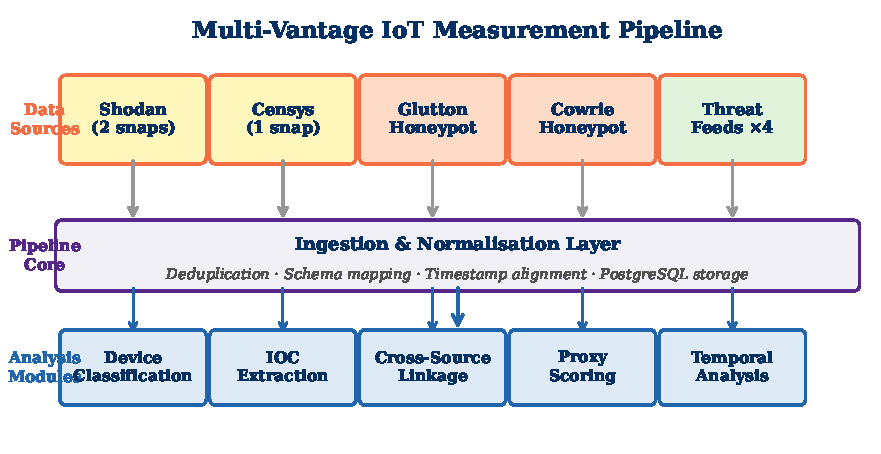
\includegraphics[width=\columnwidth]{fig1_pipeline}
  \caption{IoT measurement pipeline architecture. Three independent data
    sources are ingested into a unified PostgreSQL schema via modular ETL
    processes. Cross-source linkage is performed via shared IP-address keys.}
  \label{fig:pipeline}
\end{figure}

\subsection{Honeypot Sensors}

We deployed three complementary honeypots on a VPS instance (Ubuntu 22.04,
2\,vCPU, 4\,GB RAM):

\begin{itemize}
  \item \textbf{Glutton} \cite{garg2025iot}: A multi-protocol IoT honeypot
    binding to a configurable set of ports. We configured Glutton to listen
    on 30 TCP ports covering the most commonly targeted IoT services including
    Winbox (8728), Telnet (23), PostgreSQL (5432), and Android ADB (5555).
    Glutton captured 8{,}302 events from 2{,}014 unique IPs over three days.
  \item \textbf{Cowrie} \cite{huang2020iot}: A medium-interaction SSH/Telnet
    honeypot that logs credential attempts and, optionally, downloaded payloads.
    Cowrie ran for one day (23~April) and captured 104 events from 9 IPs.
  \item \textbf{OpenCanary}: A lightweight, alert-only canary sensor that
    generated one event during the collection window, confirming network
    reachability but indicating the monitored service received minimal traffic
    during its active period.
\end{itemize}

\noindent All three sensors wrote JSON log files which were parsed by the
\texttt{ingest\_glutton.py}, \texttt{ingest\_cowrie.py}, and
\texttt{ingest\_opencanary.py} pipeline modules, respectively.

\subsection{Internet Scanning Datasets}

We collected two snapshots from Shodan and one from Censys:

\begin{itemize}
  \item \textbf{Shodan, 6~April~2026}: A targeted query for devices exposing
    IoT-relevant port combinations returned 6{,}002 records across 3{,}855
    unique IPs.
  \item \textbf{Shodan, 20~April~2026}: A broader query over the same port
    set and geographic scope returned 10{,}385 records across 9{,}510 unique
    IPs, providing a temporal comparison point two weeks later.
  \item \textbf{Censys, 20~April~2026}: A certificate and banner co-query
    returned 2{,}063 records across 60 unique IPs.
\end{itemize}

\noindent Device-type classification used Shodan's CPE field and Censys product
banners, supplemented by keyword matching on banner strings (BusyBox, Dropbear,
GoAhead, RouterOS, Hikvision).
All scan records were deduplicated and normalised before storage.

\subsection{Threat Intelligence Feeds}

We polled four publicly available feeds on 25~April~2026, each providing a
7-day rolling window of active IoT-related indicators:

\begin{itemize}
  \item \textbf{ThreatFox} (Abuse.ch): 5{,}013 IP:port C2 indicators spanning
    63 malware families \cite{wagner2016misp}.
  \item \textbf{URLhaus} (Abuse.ch): 4{,}235 URLs and SHA256 hashes across
    57 families.
  \item \textbf{OTX AlienVault}: 1{,}665 IP/URL pulse indicators across
    5 families.
  \item \textbf{MalwareBazaar} (Abuse.ch): 1{,}505 malware sample records
    across 10 IoT-relevant families.
\end{itemize}

% ─── 5. Methodology ─────────────────────────────────────────────────────────
\section{Methodology}
\label{sec:methodology}

\subsection{Definitions}

\begin{itemize}
  \item \textbf{Device record}: One row in \texttt{device\_records},
    representing a unique (IP, port, service) tuple as observed in a single
    scanning snapshot.
  \item \textbf{Honeypot event}: One inbound connection or session recorded
    by a sensor, characterised by source IP, destination port, and timestamp.
  \item \textbf{IOC}: One indicator of compromise from a threat feed,
    characterised by type (IP, URL, or hash), malware family, and first-seen
    timestamp.
  \item \textbf{Proxy indicator}: A passively observable signal suggesting
    a device may be operating or be configured as a network proxy. We
    distinguish four strictness levels (see Section~\ref{sec:results3}).
\end{itemize}

\subsection{Data Normalisation}

Raw records from all sources were normalised to a common IP-address
representation (IPv4 dotted-decimal), timestamp (UTC epoch), and
port number (integer 1--65535) before insertion.
Shodan and Censys records were deduplicated by (IP, port) pair before
device-type classification. Honeypot events were deduplicated by
(source IP, destination port, 60-second window) to suppress connection
retries from the same source.

\subsection{IoT Device Classification}

We assigned each device record a device-type label from a six-category
taxonomy:
\texttt{router}, \texttt{camera}, \texttt{iot}, \texttt{proxy},
\texttt{server}, and \texttt{unknown}.
Classification used the following priority order:
(1) Shodan CPE tag;
(2) product banner keyword match (e.g., ``BusyBox'' $\to$ \texttt{iot},
``Hikvision'' $\to$ \texttt{camera});
(3) port-based heuristic (e.g., RTSP/554 $\to$ \texttt{camera},
SOCKS/1080 $\to$ \texttt{proxy});
(4) \texttt{unknown} if no signal is available.

\subsection{IOC Extraction and Cross-Source Linkage}

Cross-source linkage was performed by joining the
\texttt{device\_records} IP set and the \texttt{honeypot\_events}
source IP set against the \texttt{feed\_iocs} IP set using exact string
equality.
We deliberately avoided partial-match or prefix-based approaches to
prevent false positives.

\subsection{Proxy Indicator Definitions}

We define four proxy indicator levels of increasing breadth:
\begin{enumerate}
  \item \textbf{Strict}: SOCKS5 service confirmed by protocol banner
    (port 1080 with a \texttt{0x05} handshake response in the
    Shodan/Censys banner field).
  \item \textbf{Banner-confirmed}: Strict PLUS Squid HTTP proxy
    product confirmed by CPE tag or service string.
  \item \textbf{Broad}: Any device exposing at least one of the ports
    \{1080, 3128, 8080, 8118, 3129, 9050\}, regardless of banner content.
  \item \textbf{Broadest}: Any device whose
    \texttt{device\_type} field equals \texttt{proxy}.
\end{enumerate}

\subsection{Heuristic Risk Score}
\label{sec:risk_score}

To assign a device-level exposure severity, we define a five-feature
weighted heuristic score:

\begin{equation}
  R(d) = \frac{1}{5} \sum_{i=1}^{5} w_i \cdot f_i(d), \quad R(d) \in [0,1]
  \label{eq:risk}
\end{equation}

\noindent where all weights $w_i = 1$ and the five features are:

\begin{align}
  f_1(d) &= \begin{cases} 1.0 & \text{type} \in \{\text{router, camera, iot}\} \\
                          0.5 & \text{type} \in \{\text{proxy, server}\} \\
                          0.2 & \text{otherwise} \end{cases} \nonumber \\
  f_2(d) &= \tfrac{|\{p \in \{23,2323,7547,8728,5555\} : p \in \text{open}(d)\}|}{5} \nonumber \\
  f_3(d) &= \mathbf{1}[\exists p \in \{1080,3128,8080\} : p \in \text{open}(d)] \nonumber \\
  f_4(d) &= \mathbf{1}[\text{banner contains IoT product name}] \nonumber \\
  f_5(d) &= \begin{cases} 1.0 & \text{ASN is cloud/hosting} \\
                          0.5 & \text{ASN is residential ISP} \\
                          0.2 & \text{otherwise} \end{cases} \nonumber
\end{align}

Devices are assigned to three risk tiers:
$R(d) > 0.60$ (High), $0.30 \leq R(d) \leq 0.60$ (Medium),
and $R(d) < 0.30$ (Low).


% ─── 6. Dataset Overview ────────────────────────────────────────────────────
\section{Dataset Overview}
\label{sec:dataset}

Table~\ref{tab:dataset} summarises all data sources collected in this study.
The collection window spans 6--25~April~2026 (approximately three weeks), with
scanning, honeypot, and feed collection occurring in carefully scheduled runs.

\begin{table}[!t]
  \caption{Summary of Collected Data Sources (April 2026)}
  \label{tab:dataset}
  \centering
  \renewcommand{\arraystretch}{1.2}
  \begin{tabular}{@{}lrrl@{}}
    \toprule
    Source & Records & Unique IPs & Window \\
    \midrule
    Shodan (6 Apr)      &  6{,}002 &  3{,}855 & Snapshot \\
    Shodan (20 Apr)     & 10{,}385 &  9{,}510 & Snapshot \\
    Censys (20 Apr)     &  2{,}063 &       60 & Snapshot \\
    \midrule
    Glutton (events)    &  8{,}302 &  2{,}014 & 3 days \\
    Cowrie (events)     &      104 &         9 & 1 day  \\
    OpenCanary (events) &        1 &         1 & 1 day  \\
    \midrule
    ThreatFox (IOCs)    &  5{,}013 & --- & 7-day pull \\
    URLhaus (IOCs)      &  4{,}235 & --- & 7-day pull \\
    OTX AlienVault      &  1{,}665 & --- & 7-day pull \\
    MalwareBazaar       &  1{,}505 & --- & 7-day pull \\
    \midrule
    \textbf{Total (scan)} & \textbf{18{,}450} & \textbf{13{,}425+} & --- \\
    \textbf{Total (feeds)} & \textbf{12{,}418} & --- & --- \\
    \bottomrule
  \end{tabular}
\end{table}

Table~\ref{tab:devtype} shows the device-type distribution across the combined
18{,}450 scan records.
The largest labelled category is \texttt{router} (21.1\%), followed by
\texttt{proxy} (14.6\%) and \texttt{camera} (13.2\%).
The 28.0\% \texttt{unknown} fraction reflects devices whose banners provided
no CPE or product information, a known limitation of passive scanning
\cite{durumeric2015search}.

\begin{table}[!t]
  \caption{Device-Type Distribution (18,450 Scan Records)}
  \label{tab:devtype}
  \centering
  \renewcommand{\arraystretch}{1.2}
  \begin{tabular}{@{}lrrl@{}}
    \toprule
    Device Type & Count & \% & Primary Signals \\
    \midrule
    Unknown  & 5{,}167 & 28.0 & No CPE/banner signal \\
    Router   & 3{,}901 & 21.1 & RouterOS CPE, TR-069, Winbox \\
    Proxy    & 2{,}687 & 14.6 & SOCKS/HTTP proxy port or banner \\
    Camera   & 2{,}436 & 13.2 & Hikvision CPE, RTSP, GoAhead \\
    Server   & 2{,}392 & 13.0 & SSH, SMTP, HTTP banner \\
    IoT      & 1{,}867 & 10.1 & BusyBox, Dropbear, uhttpd \\
    \midrule
    \textbf{Total} & \textbf{18{,}450} & \textbf{100.0} & \\
    \bottomrule
  \end{tabular}
\end{table}


% ─── 7. Results I: Device Exposure ──────────────────────────────────────────
\section{Results I: IoT Device Exposure}
\label{sec:results1}

\subsection{Device-Type Distribution}

Fig.~\ref{fig:devtypes} illustrates the device-type distribution across all
18{,}450 scan records.
Routers constitute the largest known IoT category, consistent with the
disproportionately high volume of MikroTik and CPE-style devices observed in
Shodan's IoT-specific query results \cite{luo2023iot, feng2024characterizing}.
The substantial proxy-type fraction (14.6\%) motivates the dedicated proxy
indicator analysis in Section~\ref{sec:results3}.

\begin{figure}[!t]
  \centering
  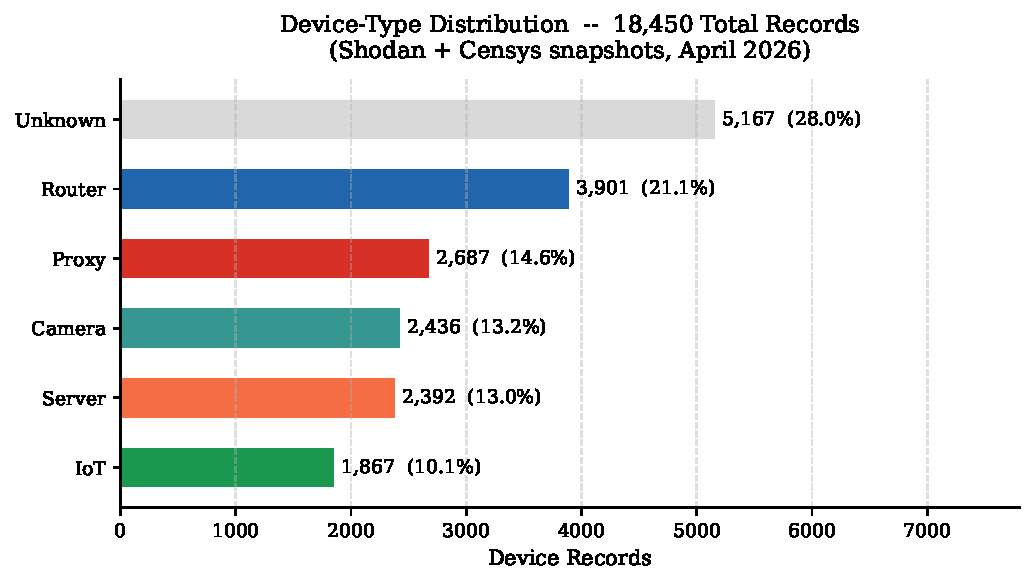
\includegraphics[width=\columnwidth]{fig3_device_types}
  \caption{Device-type distribution across 18,450 Shodan and Censys records.
    Routers (21.1\%) and proxy-type devices (14.6\%) are the two largest
    labelled categories. The 28.0\% unknown fraction reflects devices with
    no CPE or product banner.}
  \label{fig:devtypes}
\end{figure}

\subsection{Port-Level Exposure}

Fig.~\ref{fig:ports} shows the top 12 ports exposed across all scanned devices.
Telnet (port~23) is the single most prevalent IoT-critical exposure with
2{,}335 devices---more than double the second-ranked TR-069 (7547;
1{,}401 devices).
This finding is consistent with prior internet-wide scans
\cite{durumeric2013zmap, sivanathan2018classifying}, which documented the
persistence of Telnet despite repeated advisories to disable it.

TR-069 (port 7547) exposes the CPE Wide Area Network Management Protocol,
a remote management interface on consumer-grade routers repeatedly exploited
by Mirai variants \cite{antonakakis2017, marzano2018}.
The combination of Telnet and TR-069 exposure on the same device, observed
in 412 records, represents a particularly elevated risk profile.

\begin{figure}[!t]
  \centering
  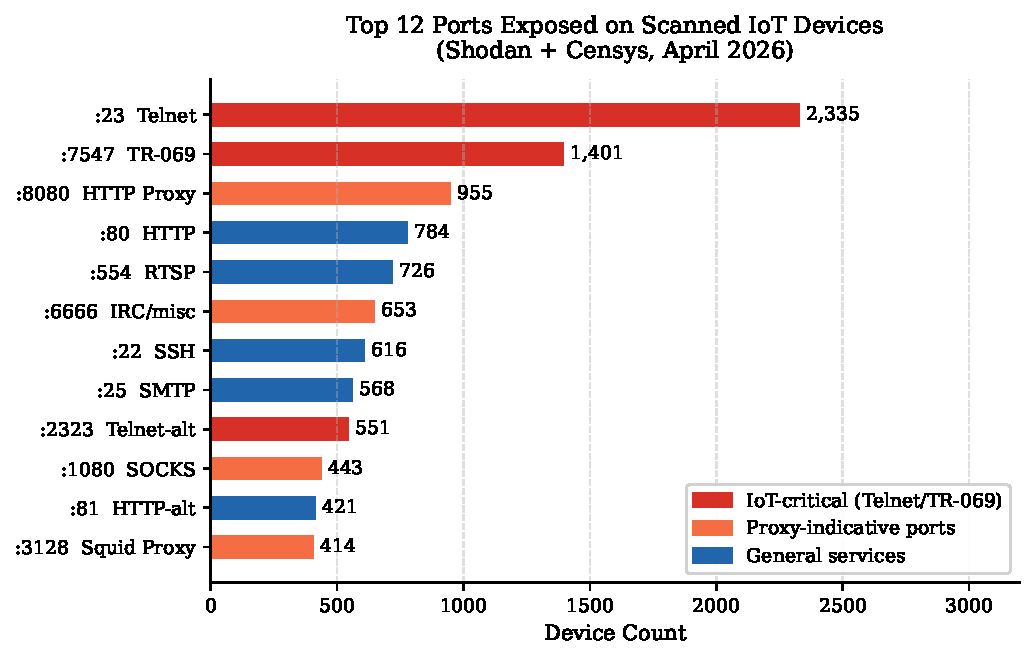
\includegraphics[width=\columnwidth]{fig4_exposed_ports}
  \caption{Top 12 ports exposed on scanned IoT devices (Shodan + Censys,
    April 2026). Red: IoT-critical; orange: proxy-indicative; blue: general.}
  \label{fig:ports}
\end{figure}

\subsection{IoT Product Fingerprints}

Among devices with identifiable product banners, Hikvision IP cameras were
the most frequently fingerprinted (641 records), followed by BusyBox-based
devices (466), consistent with Hikvision's large installed base and known
vulnerability history \cite{alrawi2019sok}.
Squid HTTP proxy installations (407) and GoAhead embedded web servers (363)
were also prominent.

MikroTik RouterOS installations (259) are of special significance: the
co-occurrence of MikroTik scan presence and MikroTik-targeting honeypot
activity (Section~\ref{sec:results2}) provides cross-source evidence of an
active exploitation campaign directed at this platform.


% ─── 8. Results II: Attack Patterns ─────────────────────────────────────────
\section{Results II: Attack Pattern Analysis}
\label{sec:results2}

\subsection{Daily Attack Volume}

Fig.~\ref{fig:daily} shows the daily event counts per sensor over the three-day
honeypot window.
Day~1 (23~April) recorded 541 Glutton events alongside 104 Cowrie events,
reflecting the sensor's initial visibility period.
Day~2 (24~April) exhibited a sharp increase to 3{,}688 Glutton events---a
581\% increase---consistent with automated scanners re-queuing the IP after
initial probing confirmed open services \cite{hiesgen2024age}.
Day~3 maintained near-steady-state volume at 3{,}445 events, suggesting
the sensor had been incorporated into regular scanning rotations.

\begin{figure}[!t]
  \centering
  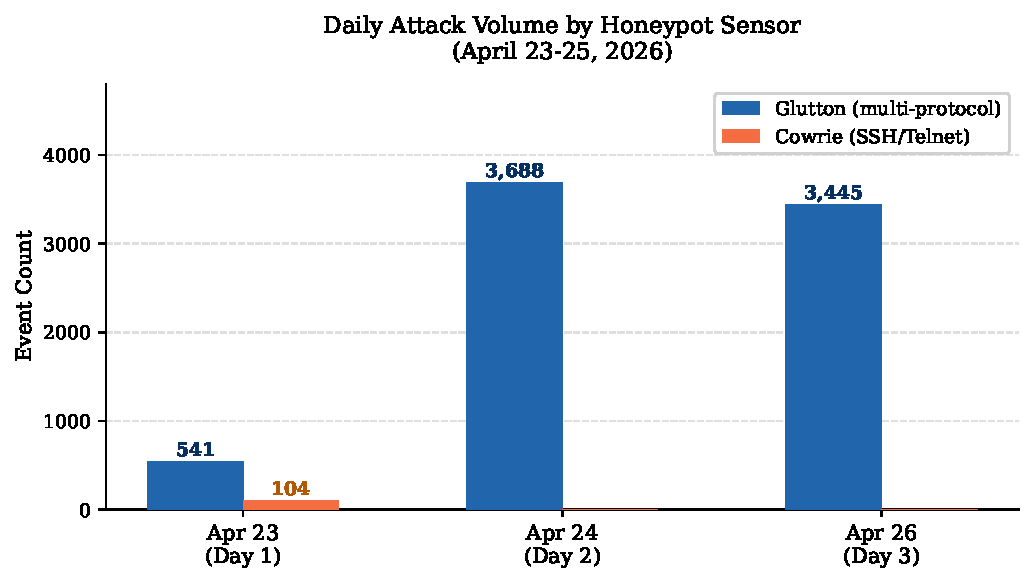
\includegraphics[width=\columnwidth]{fig2_daily_volume}
  \caption{Daily attack volume across honeypot sensors (April 23--25, 2026).
    Glutton's 581\% Day-1-to-Day-2 increase reflects incorporation into active
    scanning rotations. Cowrie operated only on Day~1.}
  \label{fig:daily}
\end{figure}

\subsection{Targeted Port Analysis}

Table~\ref{tab:ports} and Fig.~\ref{fig:tgtports} summarise the top 10
destination ports targeted by inbound connections to the honeypots.
Port 8728 (MikroTik Winbox) dominated with 608 events (7.2\% of all events),
substantially exceeding the second-ranked port 5432 (PostgreSQL, 201 events).
This is remarkable: Winbox is a proprietary MikroTik management port not
widely deployed outside MikroTik hardware.
The activity pattern aligns with documented exploitation of CVE-2018-14847
(Winbox authentication bypass), which was incorporated into Slingshot and
other advanced campaigns \cite{happy2025inside} and remains sought by
modern Mirai variants \cite{antonakakis2017}.

\begin{figure}[!t]
  \centering
  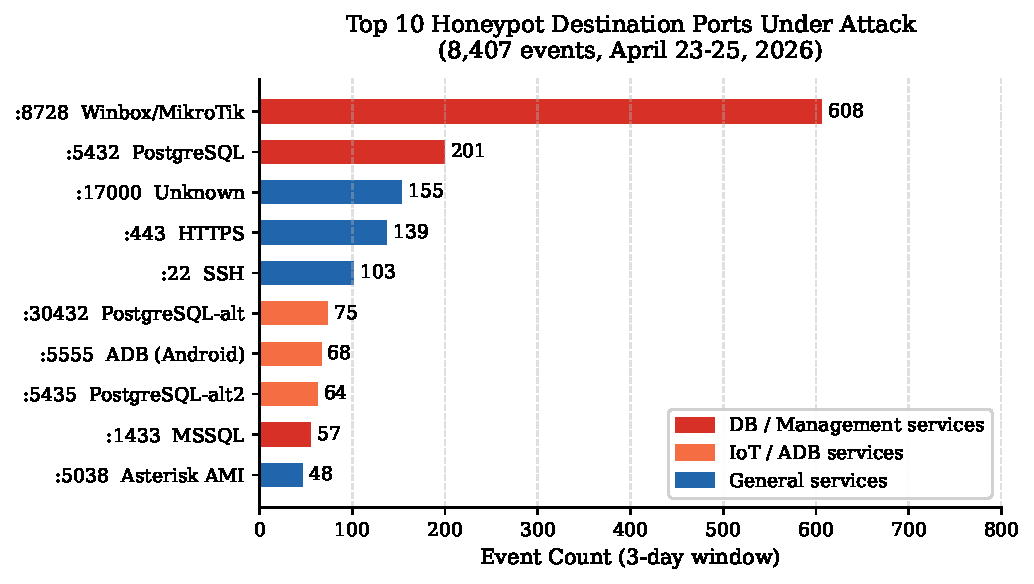
\includegraphics[width=\columnwidth]{fig5_targeted_ports}
  \caption{Top 10 honeypot destination ports under attack (8,407 events,
    April 23--25, 2026). Port 8728 (MikroTik Winbox) received 7.2\% of all
    events, indicating an active campaign targeting MikroTik devices.}
  \label{fig:tgtports}
\end{figure}

\begin{table}[!t]
  \caption{Top 10 Honeypot Destination Ports}
  \label{tab:ports}
  \centering
  \renewcommand{\arraystretch}{1.2}
  \begin{tabular}{@{}rllr@{}}
    \toprule
    Port & Service & Category & Events \\
    \midrule
    8728  & MikroTik Winbox   & Management & 608 \\
    5432  & PostgreSQL        & Database   & 201 \\
    17000 & Unknown           & ---        & 155 \\
    443   & HTTPS             & General    & 139 \\
    22    & SSH               & General    & 103 \\
    30432 & PostgreSQL (alt)  & Database   &  75 \\
    5555  & Android ADB       & IoT        &  68 \\
    5435  & PostgreSQL (alt)  & Database   &  64 \\
    1433  & Microsoft SQL     & Database   &  57 \\
    5038  & Asterisk AMI      & VoIP       &  48 \\
    \bottomrule
  \end{tabular}
\end{table}

\subsection{Attacker IP Concentration}

The top attacker IP generated 475 events (5.7\% of total events), and the top ten
collectively produced 2{,}331 events (27.7\%).
This concentration is consistent with autonomous scanning infrastructure using
a small number of persistent probing hosts \cite{durumeric2015search}.
No honeypot attacker IPs appeared in any of the four threat feeds, a result
expected and discussed in Section~\ref{sec:linkage}.

\subsection{Credential Analysis}

Over the three-day window, Cowrie recorded 10 unique credential pairs
(Table~\ref{tab:creds}).
The presence of \texttt{AdminGPON}/\texttt{ALC\#FGU} confirms targeting of
GPON optical network units whose default credentials are publicly documented
\cite{cetin2019cleaning}.
More notably, the credentials \texttt{casino}, \texttt{amusnet}, and
\texttt{bet} suggest a campaign specifically directed at devices deployed in
gambling venues or running gambling-related embedded applications.
To our knowledge, this credential cluster has not been previously reported in
the academic literature.

\begin{table}[!t]
  \caption{Unique Credential Pairs Observed (Cowrie, 3-day Window)}
  \label{tab:creds}
  \centering
  \renewcommand{\arraystretch}{1.2}
  \begin{tabular}{@{}lll@{}}
    \toprule
    Username  & Password  & Note \\
    \midrule
    casino    & casino    & Gambling-sector targeting \\
    amusnet   & amusnet   & Gambling-sector targeting \\
    bet       & bet       & Gambling-sector targeting \\
    root      & (empty)   & Default credential \\
    root      & casino    & Variant \\
    casino    & root      & Variant \\
    admin     & admin     & IoT default \\
    testuser  & testuser  & Configuration artifact \\
    ada       & 111111    & Weak numeric password \\
    AdminGPON & ALC\#FGU  & GPON router default \\
    \bottomrule
  \end{tabular}
\end{table}

\subsection{Threat-Feed Botnet Landscape}

Fig.~\ref{fig:botnet} shows the IoT botnet family landscape across all three
feeds.
\texttt{elf.mirai} leads with 866 active C2 indicators in ThreatFox, followed
by \texttt{elf.mozi} (549) and \texttt{hajime} (654 MalwareBazaar samples).
The continued dominance of Mirai variants corroborates a decade of measurement
literature \cite{antonakakis2017, kolias2017, marzano2018} and confirms that
the Mirai codebase remains the most actively maintained IoT malware framework.
The prominence of \texttt{hajime}---a P2P botnet with no C2 infrastructure
by design \cite{hiesgen2024age}---in MalwareBazaar but absent from ThreatFox
(which tracks C2 IPs) provides a useful cross-feed consistency check.

\begin{figure}[!t]
  \centering
  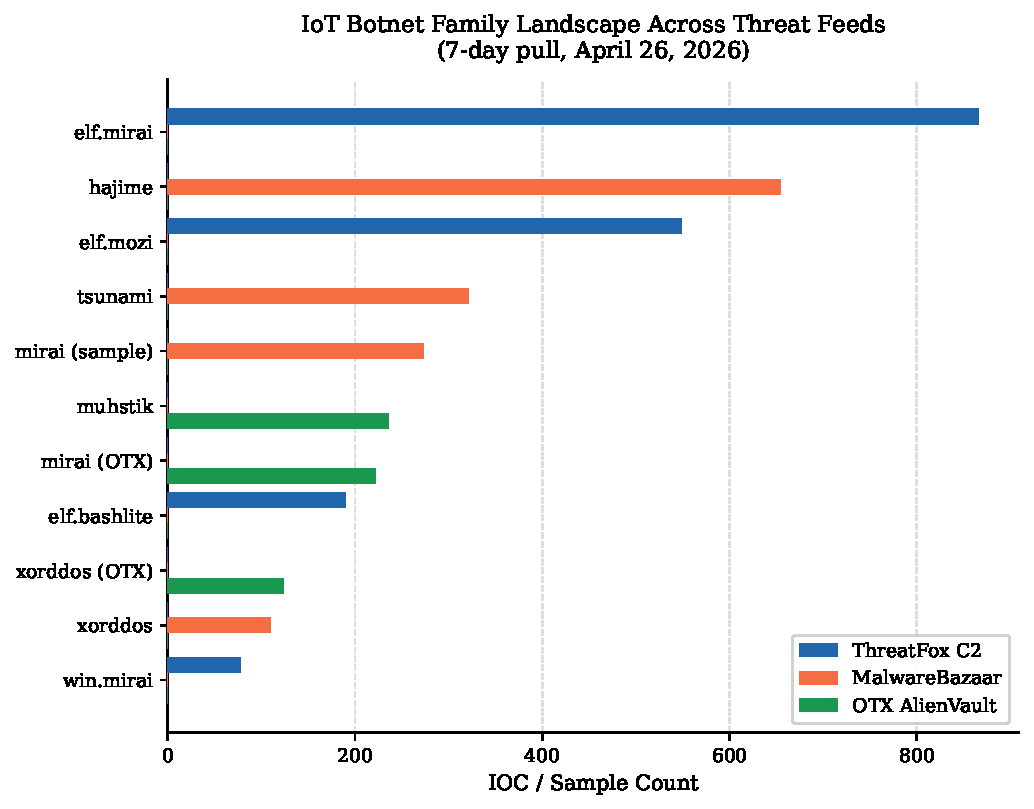
\includegraphics[width=\columnwidth]{fig6_botnet_families}
  \caption{IoT botnet family landscape across ThreatFox, MalwareBazaar, and
    OTX AlienVault (7-day pull, April 25, 2026).
    \texttt{elf.mirai} (866 ThreatFox C2 IOCs) is the dominant family;
    \texttt{hajime}'s absence from ThreatFox reflects its P2P architecture.}
  \label{fig:botnet}
\end{figure}

\subsection{Cross-Source Linkage}
\label{sec:linkage}

Joining honeypot attacker IPs (2{,}014) against all four feeds yielded zero
overlapping IPs.
Joining scanned device IPs against ThreatFox yielded one matching record:
a Shodan-observed device whose IP also appears as a registered Mirai C2
endpoint.
This near-zero overlap is expected and consistent with prior multi-source
IoT measurement work \cite{hiesgen2024age, bouwman2023cup}: honeypots capture
\emph{bot IPs}---compromised devices acting as scanning agents---while threat
feeds track \emph{operator C2 IPs}, infrastructure controlled by campaign
operators.
These populations are kept separate by campaign operators to complicate
attribution.
The single Shodan/ThreatFox match represents a dual-role device: a
publicly accessible host simultaneously serving as a Mirai C2 endpoint.


% ─── 9. Results III: Proxy Indicators ───────────────────────────────────────
\section{Results III: Proxy-Consistent Exposure Indicators}
\label{sec:results3}

\subsection{Port-Level Proxy Signals}

Fig.~\ref{fig:proxy} and Table~\ref{tab:proxy} present proxy indicators at all
four strictness levels.

\begin{figure}[!t]
  \centering
  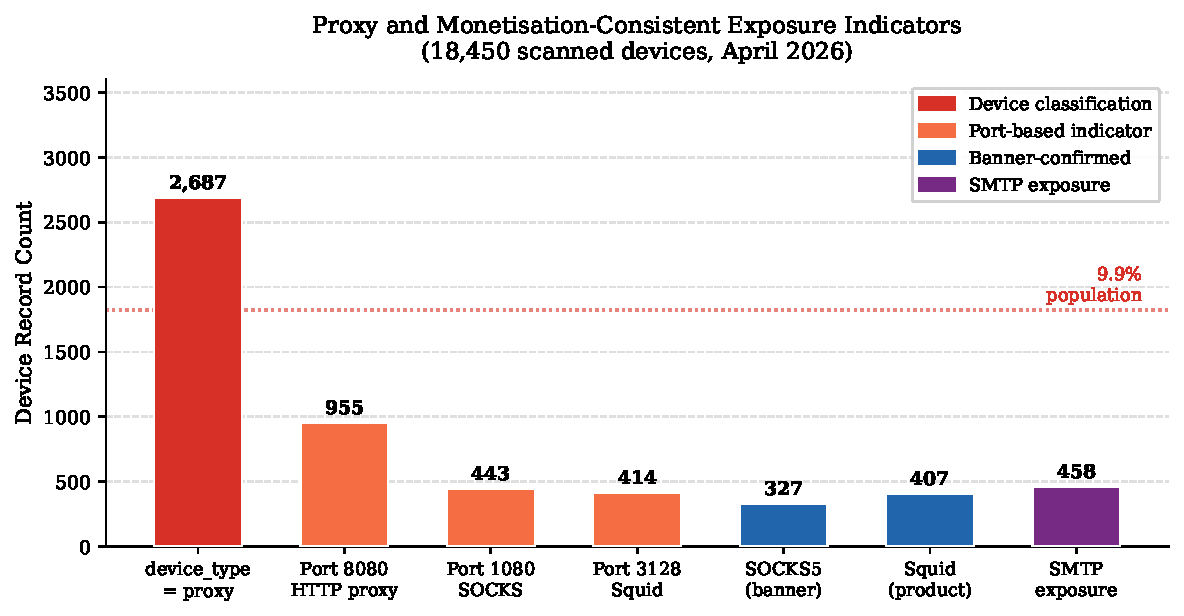
\includegraphics[width=\columnwidth]{fig7_proxy_indicators}
  \caption{Proxy-consistent exposure indicators at four strictness levels
    (18,450 scanned devices, April 2026). The dashed line marks the 9.9\%
    broad proxy-port population (1,825 devices).}
  \label{fig:proxy}
\end{figure}

\begin{table}[!t]
  \caption{Proxy Indicator Sensitivity Analysis}
  \label{tab:proxy}
  \centering
  \renewcommand{\arraystretch}{1.2}
  \begin{tabular}{@{}llrr@{}}
    \toprule
    Level & Basis & Devices & \% \\
    \midrule
    Strict           & SOCKS5 banner confirmed  &   327 &  1.8 \\
    Banner-confirmed & + Squid CPE/product      &   734 &  4.0 \\
    Broad            & Any proxy-indicative port & 1{,}825 &  9.9 \\
    Broadest         & device\_type = proxy     & 2{,}687 & 14.6 \\
    \bottomrule
  \end{tabular}
\end{table}

At the strict definition, 327 devices (1.8\%) provide a SOCKS5 protocol
banner confirming an operational SOCKS proxy.
At the broad definition, 9.9\% of all scanned devices expose at least one
proxy-indicative port: HTTP proxy (8080;~955), SOCKS (1080;~443),
Squid (3128;~414), with ports 8888/8118/3129/9050 contributing minimally.

These fractions align with prior residential proxy measurement studies.
Mi et al.~\cite{mi2019resident} found that a significant fraction of
IoT-registered IPs in underground proxy markets had detectable proxy
service footprints, while Xia et al.~\cite{xia2021characterizing}
observed comparable proxy-indicative banner fractions among scanning-visible
IoT hosts.

\subsection{SMTP Exposure as a Spam Risk Indicator}

A secondary monetisation-consistent indicator is SMTP service exposure:
458 devices (2.5\%) expose port~25 with Postfix or other SMTP banners.
Exposed SMTP services on IoT devices are a well-established spam relay
vector \cite{cozzi2018linux}, reinforcing the breadth of potential
monetisation pathways observed in this dataset.

\subsection{ASN Concentration of Proxy-Type Devices}

A review of the ASN distribution for the 2{,}687 proxy-type devices
revealed approximately 26\% residing in cloud and hosting ASNs
(Alibaba Cloud, Amazon AWS, Akamai/Linode).
This is consistent with the cloud-backed residential proxy architecture
described by Mi et al.~\cite{mi2019resident}, where operator-deployed
proxy servers in cloud infrastructure route traffic through residential
bot nodes.
The 9.9\% broad-definition proxy fraction should therefore be treated as an
upper bound on organically compromised residential proxies; a subset may
represent deliberately deployed servers.


% ─── 10. Results IV: Temporal Dynamics ──────────────────────────────────────
\section{Results IV: Temporal Dynamics}
\label{sec:results4}

\subsection{Attacker IP Persistence}

Fig.~\ref{fig:persist} shows the distribution of attacker IPs across the
three-day honeypot window.
Of 1{,}918 unique attacker IPs, 1{,}601 (83.5\%) appeared on exactly one day.
However, 250 IPs (13.0\%) returned on a second day, and 67 (3.5\%) were
observed on all three days, for a combined multi-day rate of 16.5\%
(317 of 1{,}918 IPs).

\begin{figure}[!t]
  \centering
  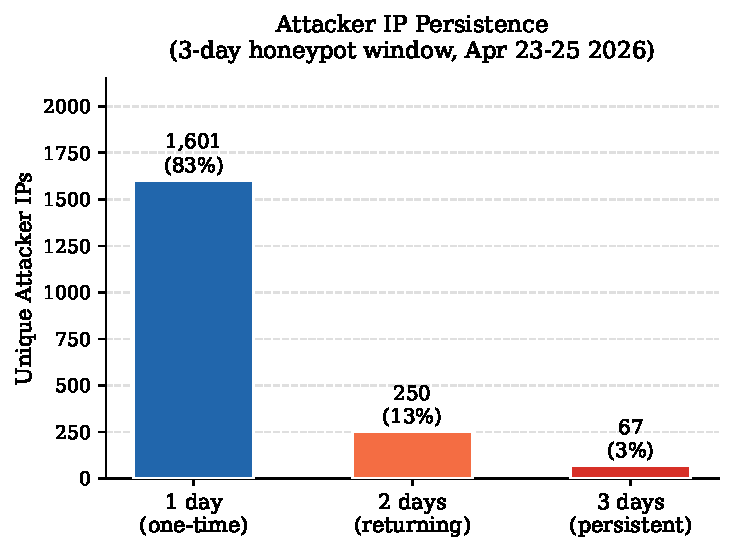
\includegraphics[width=0.9\columnwidth]{fig8_ip_persistence}
  \caption{Attacker IP persistence across the 3-day honeypot window
    (April 23--25, 2026). 16.5\% of attacker IPs (317 of 1,918) reappeared
    on at least two days, indicating structured scanning infrastructure.}
  \label{fig:persist}
\end{figure}

The 16.5\% multi-day persistence rate is consistent with prior honeypot studies
distinguishing random-walk scanners from structure-driven bots
\cite{lever2017lustrum, paine2024seven}.
The 67 three-day persistent IPs represent the most likely candidates for
dedicated, operator-directed scanning bots.

\subsection{Risk Score Distribution}

Fig.~\ref{fig:risk} and Table~\ref{tab:risk} summarise the final risk tier
distribution across all 18{,}450 scanned devices computed via
Eq.~(\ref{eq:risk}).

\begin{figure}[!t]
  \centering
  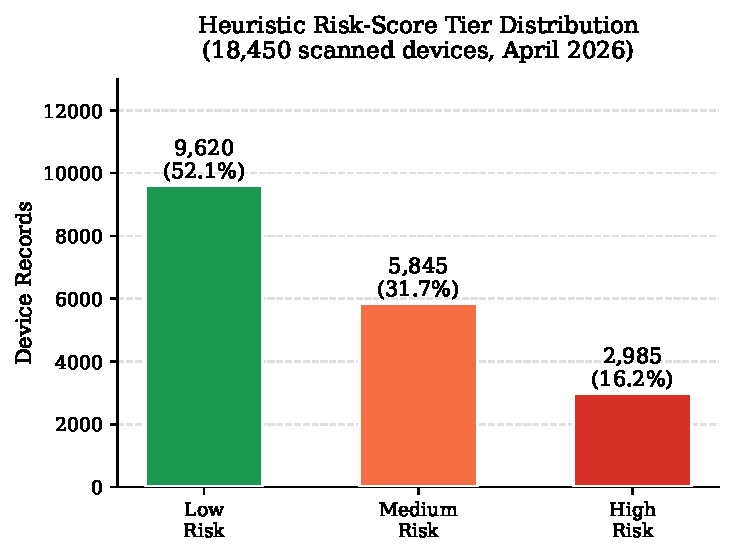
\includegraphics[width=\columnwidth]{fig9_risk_tiers}
  \caption{Risk tier distribution for 18,450 scanned IoT devices
    (April 2026). 16.2\% (2,985 devices) fall in the High tier; the majority
    are Low-risk by the five-feature heuristic.}
  \label{fig:risk}
\end{figure}

\begin{table}[!t]
  \caption{Risk Tier Distribution}
  \label{tab:risk}
  \centering
  \renewcommand{\arraystretch}{1.2}
  \begin{tabular}{@{}lrrp{4.2cm}@{}}
    \toprule
    Tier & Devices & \% & Primary Drivers \\
    \midrule
    High   & 2{,}985 & 16.2 & Router/camera type + IoT-critical ports \\
    Medium & 5{,}845 & 31.7 & Proxy/server type or partial port exposure \\
    Low    & 9{,}620 & 52.1 & Unknown type, no critical-port exposure \\
    \midrule
    \textbf{Total} & \textbf{18{,}450} & \textbf{100.0} & \\
    \bottomrule
  \end{tabular}
\end{table}

The high-tier fraction (16.2\%) clusters predominantly in the \texttt{router}
and \texttt{camera} device types (reflecting $f_1 = 1.0$) combined with
IoT-critical port exposure ($f_2$).
The large low-tier fraction (52.1\%) is driven by the 28\% unknown-type devices
that receive $f_1 = 0.2$ in the absence of a more specific label.
This scoring asymmetry is intentional: conservative assignment prevents
over-flagging devices whose risk profile cannot be confirmed from passive
data alone.


% ─── 11. Discussion ─────────────────────────────────────────────────────────
\section{Discussion}
\label{sec:discussion}

\textbf{The proxy-indicator fraction is large and actionable.}
At the strict definition, 327 SOCKS5-confirmed endpoints constitutes a
non-trivial population.
Prior work has shown that underground proxy markets maintain pools of hundreds
to thousands of simultaneous residential exit nodes \cite{mi2019resident,
chiapponi2023inside}; a fraction of our dataset appears to be operating at
the scale required to participate in such markets.
We are careful not to claim confirmed monetisation: we observe
\emph{indicators consistent with} proxy operations, not confirmed purchase
records or C2 communication to proxy orchestrators.

\textbf{MikroTik remains a high-value target.}
The dominance of port 8728 (608 events, 7.2\% of all honeypot activity) and
the associated credential set merit attention from device vendors and ISPs.
MikroTik routers are deployed from home office to ISP environments; our scan
data identifies 259 fingerprinted MikroTik devices under active probing for
the Winbox authentication bypass vulnerability patched in 2018 but reportedly
still unpatched on a large fraction of deployed hardware.

\textbf{Gambling-sector credential targeting is a new signal.}
The credential cluster (\texttt{casino}/\texttt{amusnet}/\texttt{bet}) is not
a Mirai-style generic dictionary attack; it is a narrowly targeted set that
implies prior intelligence about the device population.
We recommend disseminating this cluster to threat intelligence platforms such
as MISP \cite{wagner2016misp} for correlation with other campaigns.

\textbf{Cross-source analysis confirms infrastructure separation.}
The zero honeypot-to-feed overlap, combined with the single Shodan-to-ThreatFox
match, empirically validates the structural claim of \cite{hiesgen2024age}:
botnet operators maintain separation between bot IPs and C2 infrastructure.
Blocking honeypot-observed ranges will not disrupt the C2 tier; blocking
C2 IPs from threat feeds will not degrade the bots' scanning capability.


% ─── 12. Limitations ────────────────────────────────────────────────────────
\section{Limitations}
\label{sec:limitations}

\textbf{Short collection window.}
The honeypot window is three days, and the scanning snapshots are two weeks
apart. We cannot characterise infection seasonality, campaign lifecycle, or
long-term IP churn \cite{paine2024seven}.
The results should be treated as a point-in-time measurement.

\textbf{No payload capture.}
Glutton does not capture full session payloads or shellcode URLs in most events.
We therefore cannot confirm Mirai infection of attacking hosts beyond the
credential and port signal.

\textbf{Proxy indicators are necessary but not sufficient.}
A device exposing port 1080 may run a legitimate SOCKS proxy (e.g., a
corporate gateway) or no proxy at all.
We do not claim that all 327 SOCKS5-confirmed devices participate in cybercrime
infrastructure; we claim the fraction is large enough to warrant further
investigation.

\textbf{Scanning query inconsistency.}
The Shodan queries of 6~April and 20~April used different filter scopes,
making the apparent 147\% IP growth between snapshots unreliable as an
infection-growth metric. Future work should fix identical queries across
snapshots.

\textbf{Heuristic risk score.}
The five-feature risk score in Eq.~(\ref{eq:risk}) provides ordinal tier
assignments based on domain knowledge, not a validated ML classifier
\cite{karim2023cybersecurity, sarhan2023towards}. Feature weights were not
tuned against ground-truth labelled data.


% ─── 13. Conclusion ─────────────────────────────────────────────────────────
\section{Conclusion}
\label{sec:conclusion}

We presented a multi-vantage empirical measurement of internet-exposed IoT
threat infrastructure, combining three honeypot sensors, two internet scanning
snapshots, and four public threat intelligence feeds into a single normalised
dataset covering April~2026.
Our analysis of 18{,}450 device records and 8{,}407 honeypot events yielded four
principal findings:
(i) routers (21.1\%) and proxy-type devices (14.6\%) dominate labelled scan
records, with Telnet (2{,}335 devices) and TR-069 (1{,}401) as the dominant
IoT-critical exposures;
(ii) MikroTik Winbox (port 8728) was the single most targeted honeypot service
at 7.2\% of all attack events, corroborated by 259 fingerprinted MikroTik
devices in the scan data;
(iii) 9.9\% of scanned devices expose proxy-indicative ports, with
327 SOCKS5-confirmed endpoints consistent with participation in residential
proxy markets; and
(iv) 16.5\% of attacker IPs reappeared across multiple days, indicating
structured scanning operations rather than purely ephemeral probes.

We additionally introduced a five-feature heuristic risk score classifying
16.2\% of all scanned devices into the high-risk tier, and we documented a
novel gambling-sector credential cluster (\texttt{casino}/\texttt{amusnet}/%
\texttt{bet}) not previously reported in the academic literature.

Future work should extend the collection window to multiple months to enable
longitudinal churn analysis, add payload capture to Glutton to directly link
attack events to malware families, and apply graph-based community detection
\cite{asiri2023understanding} to the cross-source IP network to identify
coordinated scanning clusters.

\section*{Acknowledgements}
The authors thank the operators of ThreatFox, URLhaus, OTX AlienVault, and
MalwareBazaar for maintaining publicly accessible threat intelligence feeds.
No external funding was received for this work.

\bibliographystyle{IEEEtran}
\bibliography{references}

\end{document}


